%
% ground_segment.tex
%
% Copyright (C) 2021 by SpaceLab.
%
% FloripaSat-2 Documentation
%
% This work is licensed under the Creative Commons Attribution-ShareAlike 4.0
% International License. To view a copy of this license,
% visit http://creativecommons.org/licenses/by-sa/4.0/.
%

%
% \brief Ground segment chapter.
%
% \author Gabriel Mariano Marcelino <gabriel.mm8@gmail.com>
%
% \institution Universidade Federal de Santa Catarina (UFSC)
%
% \version 0.1.0
%
% \date 2020/06/06
%

\chapter{Ground Segment} \label{ch:ground-segment}

This chapter describes the ground segment of the mission. It is composed by two ground stations (one at the INPE-RN installations and other at the SpaceLab installations) and many data collection platforms (PCD\nomenclature{\textbf{PCD}}{\textit{``Plataforma de Coleta de Dados'', or Data Collection Platform}}, or \textit{``Plataforma de Coleta de Dados''}), installed at a variety of locations on the brazilian territory.

The control of the mission and the reception of the collected data will be performed mainly at these two ground stations, but if necessary, other stations can execute this task. The amateur radio link can be used by any station in the world since having the required equipment to it.

\section{UFSC Ground Station}

The UFSC ground station is currently being developed and prepared for this mission. This section presents the project of this station. A general block diagram can be seen in \autoref{fig:grs-block-diagram}.

\begin{figure}[!ht]
    \begin{center}
        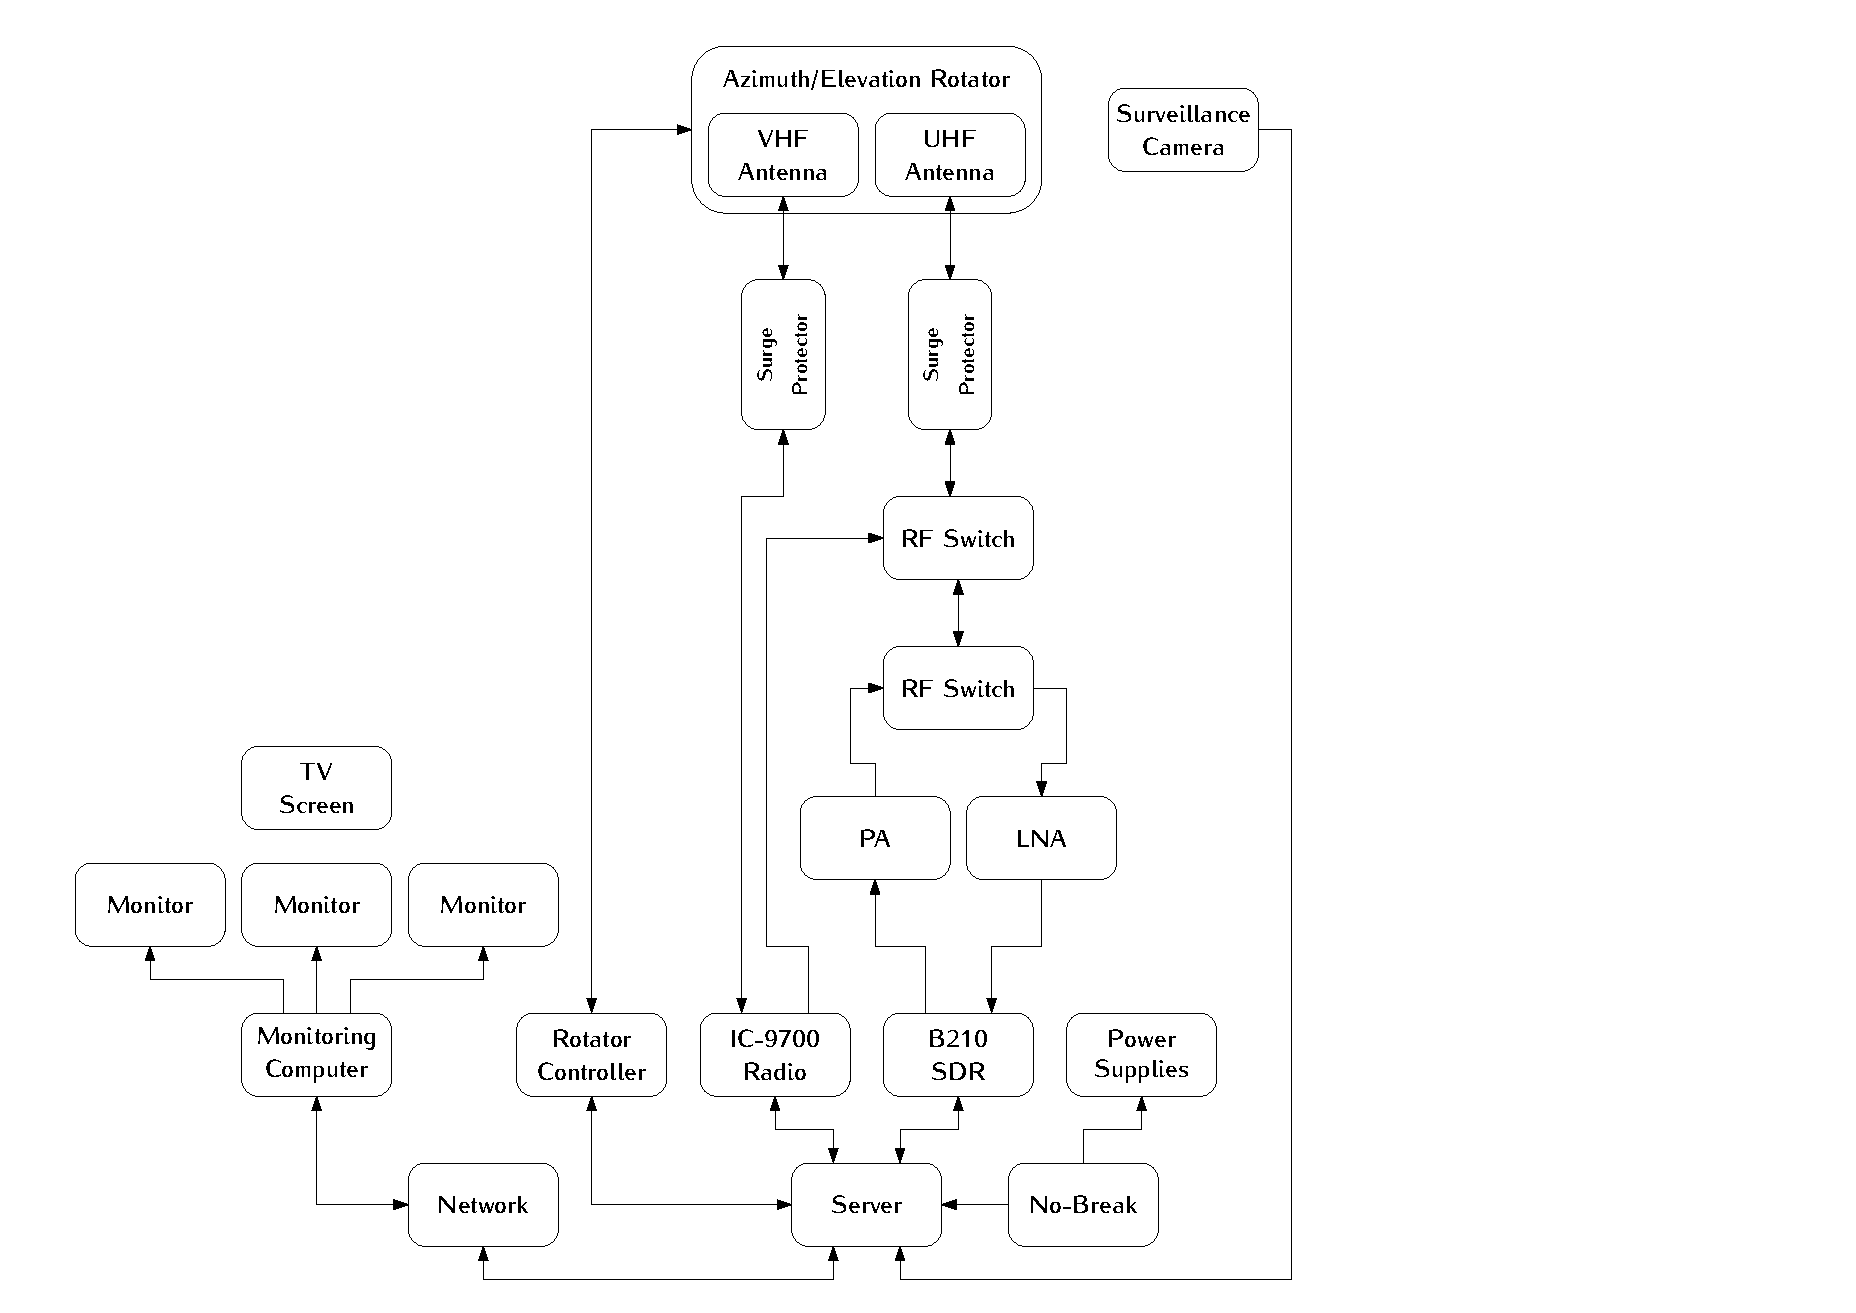
\includegraphics[width=\textwidth]{figures/grs-block-diagram.pdf}
        \caption{Block diagram of the ground segment.}
        \label{fig:grs-block-diagram}
    \end{center}
\end{figure}

In the next sections, a description of the main components of the station will be presented.

\subsection{Hardware}

\subsubsection{Antennas}

There are two antennas in the ground station: One for VHF and one for the UHF band. The main characteristics of these antennas can be seen in \autoref{tab:grs-antennas}

\begin{table}[ht]
    \centering
    \begin{tabular}{lccc}
        \toprule[1.5pt]
        \textbf{Characteristic} & \textbf{VHF Antenna}  & \textbf{UHF Antenna}  & \textbf{Unit} \\
        \midrule
        Brand                   & M$^{2}$               & Cushcraft             & - \\
        Model                   & 2MCP14                & A719B                 & - \\
        Type                    & Yagi                  & Yagi                  & - \\
        Number of elements      & 14                    & 19                    & - \\
        Frequency range         & 143-148               & 430-450               & MHz \\
        Gain                    & 12,34                 & 15,5                  & dBi \\
        Power rating            & 1500                  & 2000                  & W \\
        Boom length             & 3,2                   & 4,1                   & m \\
        Longest element         & 1,02                  & 0,34                  & m \\
        Weight                  & 2,72                  & 2,55                  & kg \\
        \bottomrule[1.5pt]
    \end{tabular}
    \caption{Main characteristics of the ground segment antennas.}
    \label{tab:grs-antennas}
\end{table}

More information about the VHF and UHF antennas can be found in \cite{2mcp14} and \cite{a719b} respectively.

\paragraph{Surge Protector}

.

\subsubsection{Rotators}

Both antennas (VHF and UHF) track the satellite through a two axis rotator (azimuth and elevation). The used model is the Yaesu G-5500, which provides 450$^{\circ}$ azimuth and 180$^{\circ}$ elevation control of medium and large size unidirectional satellite antenna arrays under remote control from station operation position.

A picture of the G-5500 rotator (and controller) can be seen in \autoref{fig:g5500}, the main characteristics can be found in \autoref{tab:grs-rotor}.

\begin{figure}[!ht]
    \begin{center}
        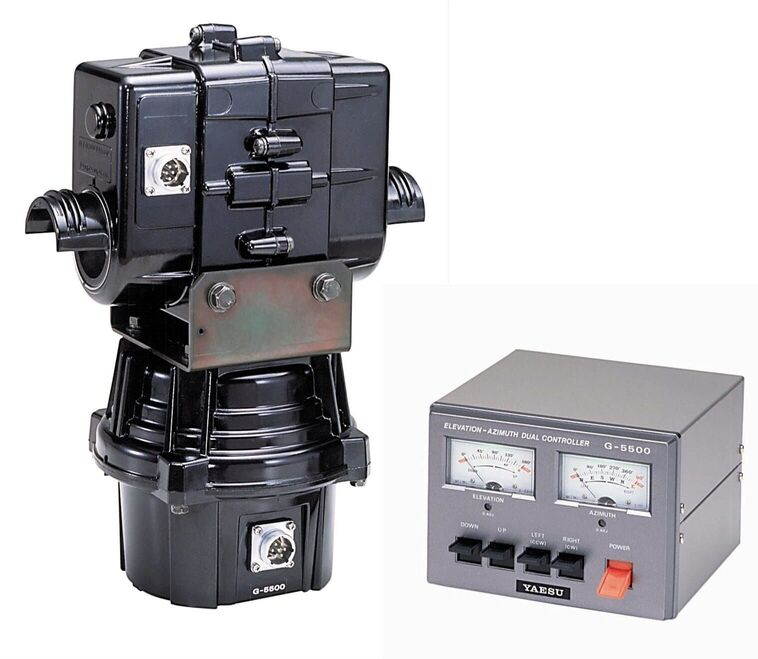
\includegraphics[width=0.6\textwidth]{figures/g5500.jpg}
        \caption{Yaesu G-5500 rotator and controller.}
        \label{fig:g5500}
    \end{center}
\end{figure}

\begin{table}[ht]
    \centering
    \begin{tabular}{lcc}
        \toprule[1.5pt]
        \textbf{Characteristic}                     & \textbf{Value}        & \textbf{Unit} \\
        \midrule
        Brand                                       & Yaesu                 & - \\
        Model                                       & G-5500                & - \\
        Voltage requirement                         & 110-120 or 200-240    & $V_{AC}$ \\
        Motor voltage                               & 24                    & V$_{AC}$ \\
        Rotation time (elevation, 180$^{\circ}$)    & 67                    & s \\
        Rotation time (azimuth, 360$^{\circ}$)      & 58                    & s \\
        Maximum continuous operation                & 5                     & min \\
        Rotation torque (elevation)                 & 14                    & kg-m \\
        Rotation torque (azimuth)                   & 6                     & kg-m \\
        Braking torque (elevation and azimuth)      & 40                    & kg-m \\
        Vertical load                               & 200                   & kg \\
        Pointing accuracy                           & $\pm$ 4               & \% \\
        Wind surface area                           & 1                     & $m^{2}$ \\
        Weight (rotator)                            & 9                     & kg \\
        Weight (controller)                         & 3                     & kg \\
        \bottomrule[1.5pt]
    \end{tabular}
    \caption{Main characteristics of antennas' rotators.}
    \label{tab:grs-rotor}
\end{table}

More information about the ground station rotator can be found in \cite{g5500}.

\subsubsection{Amplifiers}

\paragraph{Power Amplifier}

PA\nomenclature{\textbf{PA}}{\textit{Power Amplifier}}...

A picture of the power amplifier can be seen in \autoref{fig:zhl-50w}, the main characteristics are available in \autoref{tab:zhl-50w-specs}.

\begin{figure}[!ht]
    \begin{center}
        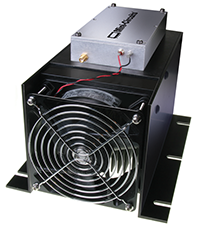
\includegraphics[width=0.3\textwidth]{figures/zhl-50w.png}
        \caption{Mini-Circuits ZHL-50W-52-S+ power amplifier.}
        \label{fig:zhl-50w}
    \end{center}
\end{figure}

\begin{table}[ht]
    \centering
    \begin{tabular}{lcc}
        \toprule[1.5pt]
        \textbf{Characteristic} & \textbf{Value}    & \textbf{Unit} \\
        \midrule
        Brand                   & Mini-Circuits     & - \\
        Model                   & ZHL-50W-52-S+     & - \\
        Frequency range         & 50-500            & MHz \\
        Gain                    & 47-52             & dB \\
        Noise figure            & 4,5-7,0           & dB \\
        DC supply voltage       & 24-25             & V \\
        Max. supply current     & 9,3               & A \\
        \bottomrule[1.5pt]
    \end{tabular}
    \caption{Main characteristics of the ZHL-50W-52-S+ power amplifier.}
    \label{tab:zhl-50w-specs}
\end{table}

\paragraph{Low Noise Amplifiers}

LNA\nomenclature{\textbf{LNA}}{\textit{Low Noise Amplifier.}}...

\subsubsection{Radios}

The Icom IC-9700 \cite{ic9700} is an RF direct sampling receiver for 2 m and 70 cm. The IF receiver consists of a single, down conversion for 23 cm that is between 311 and 371 MHz. The PA provides 100 W on 2 m, 75 W on 70 cm, and 10 W on 23 cm.

In addition to band specific memory channels, the IC-9700 allows band specific receiver and transmitter settings. For transmit, users can make adjustments to RF power, TX power Limit, Limit Power, and TX Delay by band. Basic receiver settings, like the Noise Blanker, Noise Reduction, and others can be tweaked by band with a dynamic Notch and Filter setup by band/mode.

A picture of the IC-9700 radio can be seen in \autoref{fig:ic9700}.

\begin{figure}[!ht]
    \begin{center}
        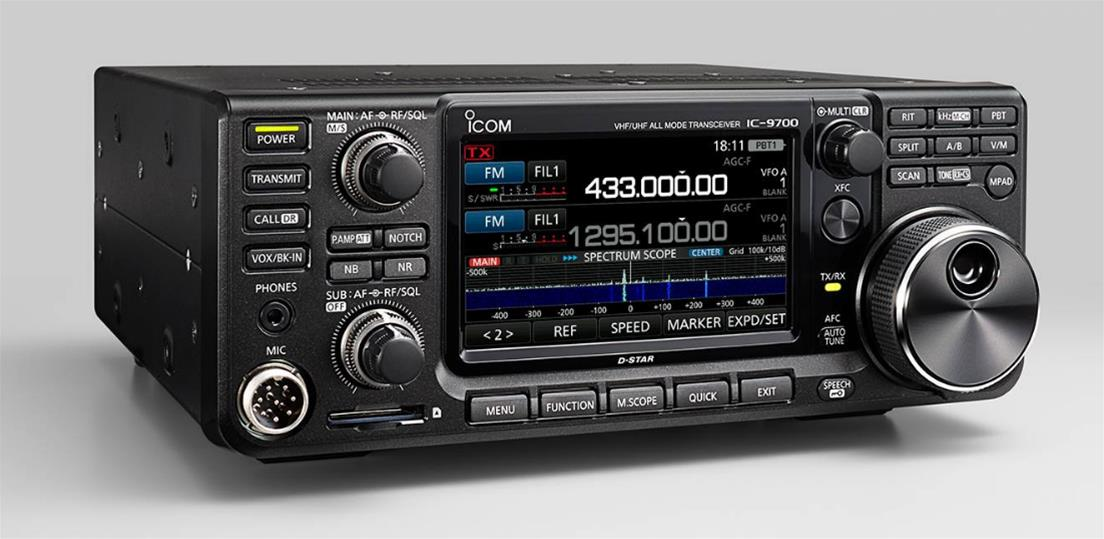
\includegraphics[width=0.7\textwidth]{figures/ic-9700.jpg}
        \caption{Icom IC-9700 radio transceiver.}
        \label{fig:ic9700}
    \end{center}
\end{figure}

\paragraph{Software Defined Radio}

As presented in \autoref{fig:grs-block-diagram}, the ground segment also has an SDR\nomenclature{\textbf{SDR}}{\textit{Software Defined Radio.}} (Software Defined Radio) as transceiver. The used model is the USRP B210, from Ettus Research \cite{b210}, which is a fully integrated, single-board SDR with continuous frequency coverage from 70 MHz to 6 GHz. It combines the AD9361 RFIC direct-conversion transceiver providing up to 56 MHz of real-time bandwidth, an open and reprogrammable Spartan6 FPGA, and USB 3.0 connectivity. Also, a full support for the USRP Hardware Driver (UHD) software allows the use with the GNURadio framework.

A picture of the USRP B210 SDR (with enclosure) can be seen in \autoref{fig:usrp-b210}.

\begin{figure}[!ht]
    \begin{center}
        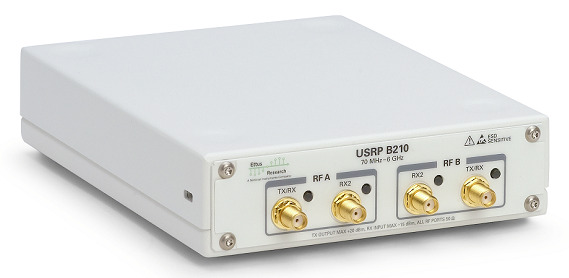
\includegraphics[width=0.6\textwidth]{figures/usrp-b210.jpg}
        \caption{Ettus USRP B210 SDR.}
        \label{fig:usrp-b210}
    \end{center}
\end{figure}

\subsubsection{Processing and Control}

.

\subsection{Satellite Tracking}

To track the satellite and for orbit prediction, the GPredict software \cite{gpredict} will be used. Gpredict is a real-time satellite tracking and orbit prediction application. It can track a large number of satellites and display their position and other data in lists, tables, maps, and polar plots (radar view). Gpredict can also predict the time of future passes for a satellite, and provide you with detailed information about each pass. Gpredict is free software licensed under the GNU General Public License. A picture of the main window of GPredict can be seen in \autoref{fig:gpredict}.

\begin{figure}[!ht]
    \begin{center}
        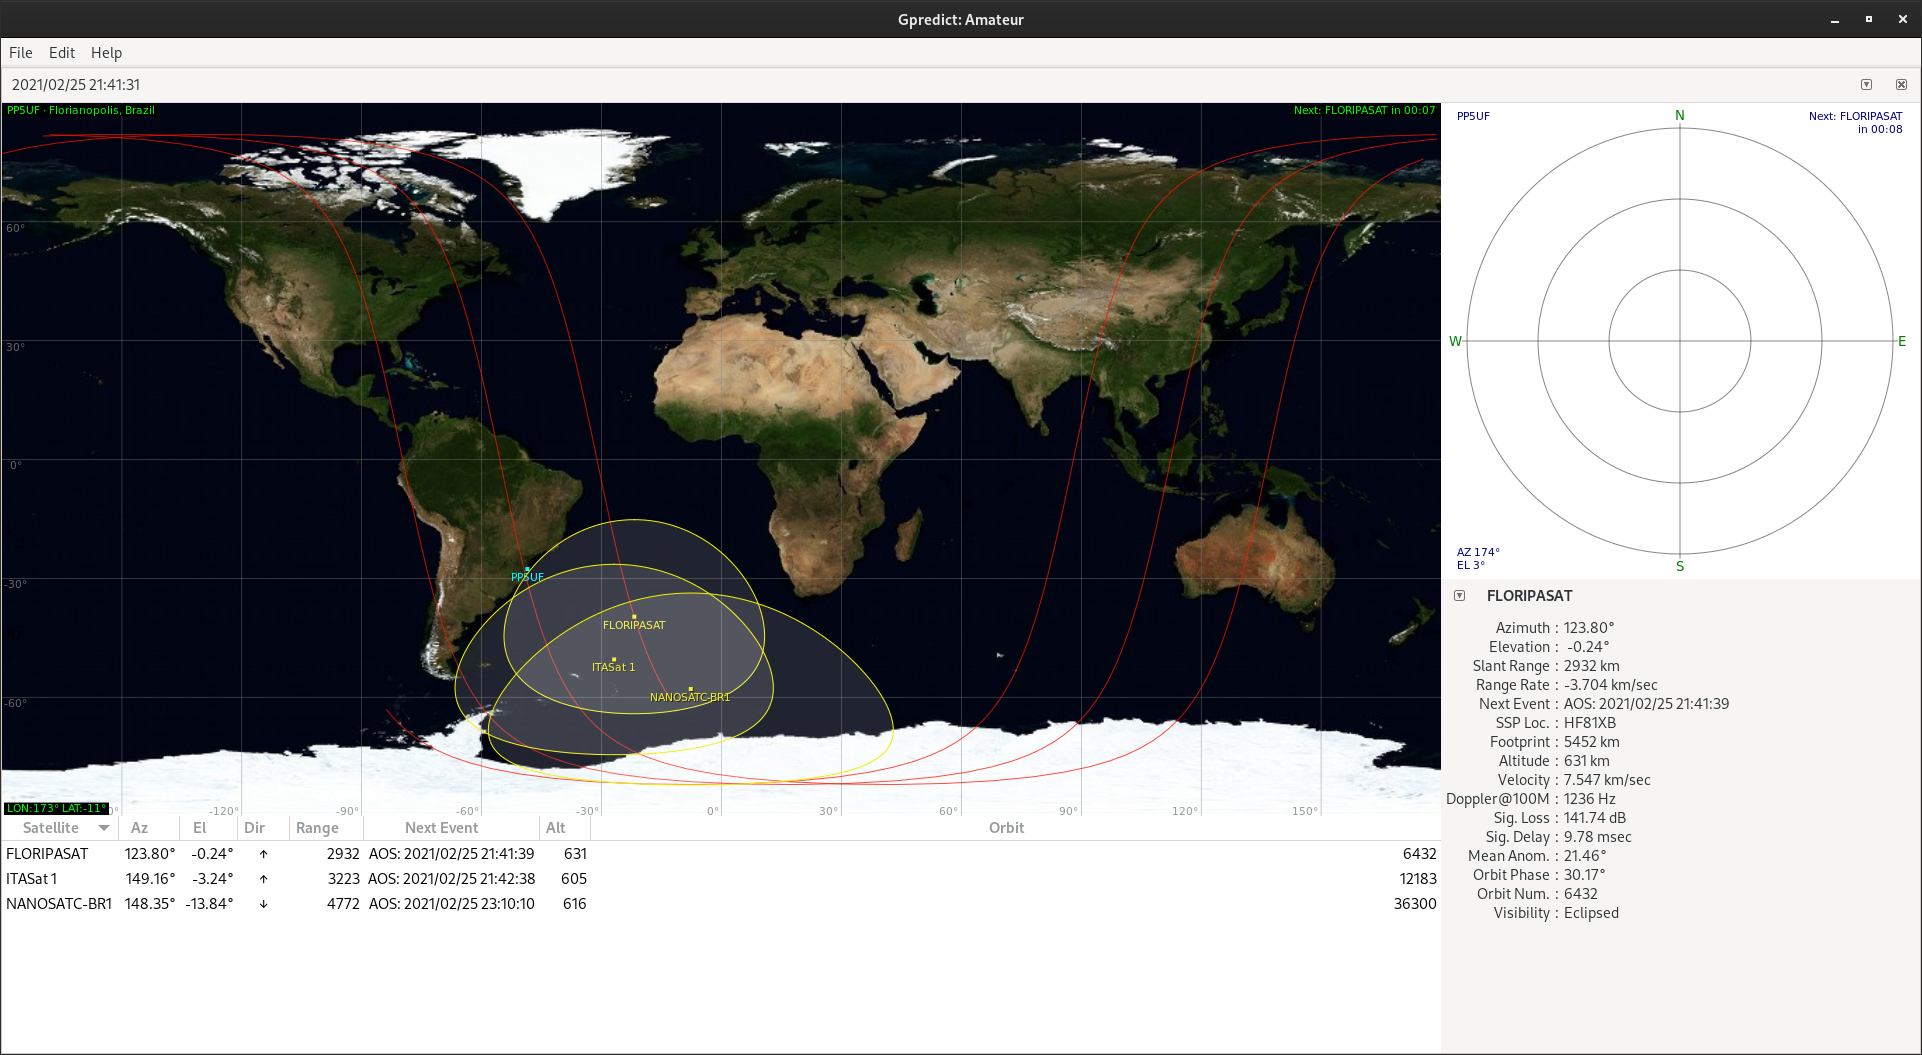
\includegraphics[width=\textwidth]{figures/gpredict.png}
        \caption{Main window of GPredict.}
        \label{fig:gpredict}
    \end{center}
\end{figure}

\subsection{Packet Decoding}

\cite{spacelab-decoder}

\begin{figure}[!ht]
    \begin{center}
        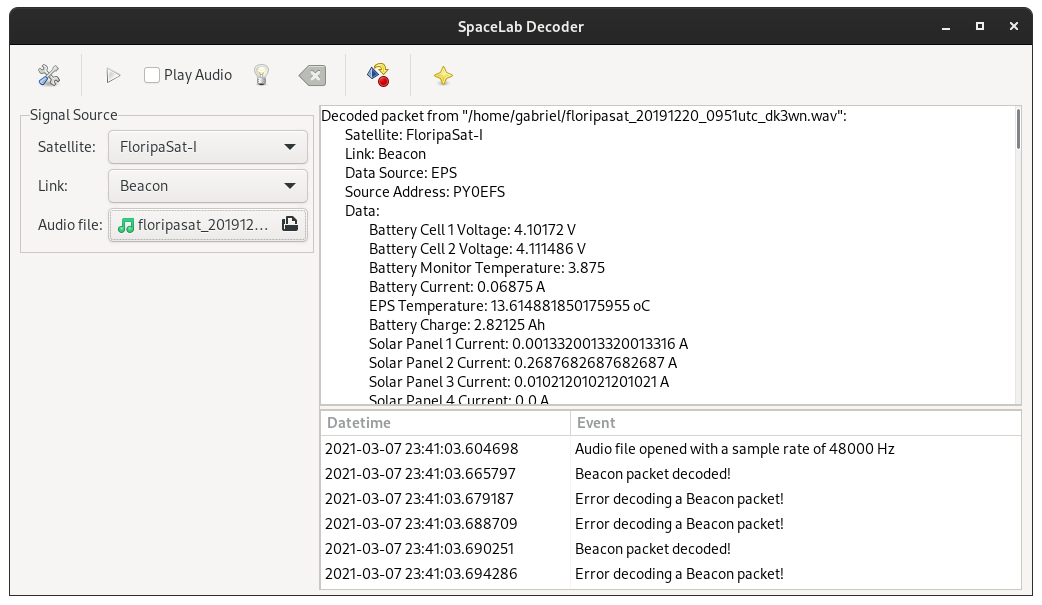
\includegraphics[width=\textwidth]{figures/spacelab-decoder.png}
        \caption{Main window of the SpaceLab Decoder application.}
        \label{fig:spacelab-decoder}
    \end{center}
\end{figure}

\section{INPE-RN Ground Station}

.

\section{Data Collection Platforms (PCDs)}

.
